\documentclass[aspectratio=169,10pt]{beamer}
\usetheme[progressbar=frametitle,numbering=fraction,block=fill]{metropolis}
\setbeamercolor{background canvas}{bg=white}
\usepackage[T1]{fontenc}
\usepackage{booktabs}
\usepackage{graphicx}
\usepackage{amsmath,amssymb}
\graphicspath{{../figures/}}
% Generated by xaibench.stats.report.findings_macros -- do not edit.
\newcommand{\ProfileName}{FULL}
\newcommand{\NumCells}{18}
\newcommand{\NumExplained}{1746}
\newcommand{\MedianRho}{0.74}
\newcommand{\MedianJaccardFive}{0.67}
\newcommand{\MedianRboNorm}{0.74}
\newcommand{\RhoPima}{0.76}
\newcommand{\RhoHeart}{0.78}
\newcommand{\RhoCkd}{0.63}
\newcommand{\AucPima}{0.83}
\newcommand{\AucHeart}{0.90}
\newcommand{\AucCkd}{1.00}
\newcommand{\AopcShap}{0.260}
\newcommand{\AopcLime}{0.224}
\newcommand{\AopcRandom}{0.075}
\newcommand{\AopcBestFusion}{0.248}
\newcommand{\LipschitzShap}{0.18}
\newcommand{\LipschitzLime}{0.65}
\newcommand{\RerunCvLime}{0.68}
\newcommand{\RetrainShap}{0.83}
\newcommand{\RetrainLime}{0.76}
\newcommand{\SecondsShap}{0.0019}
\newcommand{\SecondsLime}{0.0462}
\newcommand{\SpeedFactor}{24.8}
\newcommand{\HOneRejected}{15}
\newcommand{\HOneTotal}{18}
\newcommand{\HThreeBRejected}{36}
\newcommand{\HThreeBTotal}{36}
\newcommand{\HSixRejected}{0}
\newcommand{\HSixTotal}{18}
\newcommand{\AdditivityMedianMax}{3.5e-8}
\newcommand{\AdditivityOutlierCells}{1}
\newcommand{\AdditivityGateFailCells}{1}
\newcommand{\AdditivityWorstMax}{0.094}
\newcommand{\AdditivityWorstOutliers}{5}
\newcommand{\RboFloorEight}{0.589}
\newcommand{\RboFloorThirteen}{0.416}
\newcommand{\RboFloorTwentyFour}{0.193}


\setbeamertemplate{navigation symbols}{}
\newcommand{\shap}{\textsc{shap}}
\newcommand{\lime}{\textsc{lime}}
\newcommand{\aopc}{\textsc{aopc}}
\newcommand{\RQ}[1]{RQ#1}
\newcommand{\takeaway}[1]{\vfill{\small\color{structure}\textbf{#1}}}

\title{SHAP versus LIME on Clinical Tabular Data}
\subtitle{A reproducible benchmark of agreement, stability, fidelity, and consensus}
\author{S.\,O.\ Antika \and Y.\,A.\ Shuchona \and M.\,M.\ Haque \and G.\,J.\ Tripura}
\institute{Department of Computer Science and Engineering, University of Chittagong\\
\smallskip Supervisor: Dr.\ M.\ Jamshed Alam Patwary\\
\smallskip ENG 672 --- Technical Communication and Writing}
\date{\today}

\begin{document}
\begin{frame}[plain]\titlepage\end{frame}

\begin{frame}{The models that work best on tabular data are the ones nobody can read}
\begin{columns}[T]
\begin{column}{0.54\textwidth}
\begin{itemize}\setlength\itemsep{0.6em}
  \item Tree ensembles win on tabular data --- and their reasoning is not in the weights
  \item Regulation now requires explanations, not just accuracy (EU AI Act, 2024)
  \item Two methods dominate practice: \shap{} and \lime{}
\end{itemize}
\end{column}
\begin{column}{0.44\textwidth}
\small
\begin{block}{They rest on different theory}
\shap{}: cooperative-game attribution of the output.\\[0.4em]
\lime{}: a linear surrogate fitted near one prediction.
\end{block}
\end{column}
\end{columns}
\takeaway{So they can disagree about the same prediction --- and a practitioner
who sees two different top-five lists has no principled way to choose.}
\end{frame}

\begin{frame}{Existing comparisons vary one axis, so nothing generalises}
\begin{itemize}\setlength\itemsep{0.7em}
  \item Typically \textbf{one model family}, or \textbf{one dataset}
  \item Fidelity metrics \textbf{defined differently} in every paper
  \item \textbf{No hypothesis tests}, no effect sizes, no correction for multiplicity
  \item \textbf{No random control}, so fidelity numbers have no scale
  \item Output space never stated --- often comparing log-odds against probability
\end{itemize}
\takeaway{The gap is not a missing algorithm. It is a missing controlled comparison ---
and that is something an experiment can actually close.}
\end{frame}

\begin{frame}{Our question, and what we claim}
\begin{block}{Question}
Across model families and datasets, how far do \shap{} and \lime{} agree, how stable and
faithful is each, what does each cost --- and does combining them help?
\end{block}
\medskip
\begin{enumerate}\setlength\itemsep{0.5em}
  \item A \textbf{reproducible benchmark}: \NumCells{} model--dataset cells,
    \NumExplained{} explained instances, 11 pre-registered hypotheses
  \item A \textbf{three-way decomposition of stability}: explainer randomness,
    input perturbation, model retraining
  \item A \textbf{controlled evaluation of three rank-fusion rules} against a strict bar
\end{enumerate}
\takeaway{We do not claim to have invented explanation fusion --- that exists and we
cite it. The contribution is the evaluation.}
\end{frame}

\begin{frame}{One pipeline, two deliberately separated tracks}
\begin{center}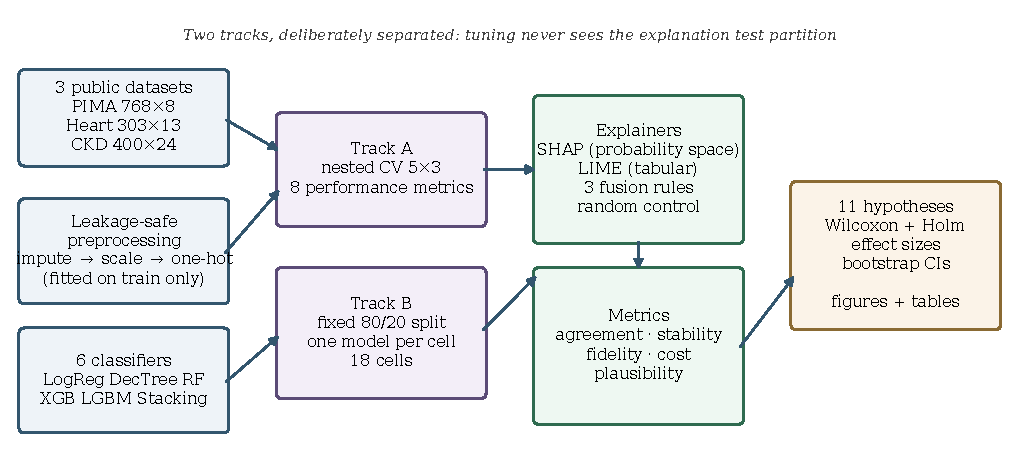
\includegraphics[width=0.95\textwidth]{F1.pdf}\end{center}
\takeaway{Track A tunes and scores. Track B explains a model whose test partition never
took part in tuning. Conflating them is how explanation studies leak.}
\end{frame}

\begin{frame}{Three datasets chosen to span a difficulty gradient}
\begin{columns}[T]
\begin{column}{0.5\textwidth}
\small
\begin{tabular}{@{}lrrr@{}}
\toprule
Dataset & $n$ & Feat. & ROC-AUC \\
\midrule
PIMA Diabetes & 768 & 8 & \AucPima{} \\
Heart Disease & 303 & 13 & \AucHeart{} \\
Chronic Kidney & 400 & 24 & \AucCkd{} \\
\bottomrule
\end{tabular}
\medskip
\footnotesize All public, de-identified, redistributable.\\
Diseases are \textbf{benchmarks}. No medical claims.
\end{column}
\begin{column}{0.5\textwidth}
\begin{itemize}\setlength\itemsep{0.4em}
  \item 6 classifiers: LogReg, DecTree, RF, XGBoost, LightGBM, Stacking
  \item 6 explainers: \shap{}, \lime{}, 3 fusion rules, \textbf{random control}
  \item 16 interpretability measures across 5 families
\end{itemize}
\end{column}
\end{columns}
\takeaway{A single dataset cannot ask whether explainer agreement depends on how hard
the decision boundary is. Three, spanning \AucPima{} to \AucCkd{}, can.}
\end{frame}

\begin{frame}{Four traps that silently invalidate this comparison}
\small
\begin{enumerate}\setlength\itemsep{0.55em}
  \item \textbf{Different output spaces.} \lime{} explains probability; tree \shap{}
    defaults to log-odds. We force probability space and \emph{verify} it by additivity
    --- median error \AdditivityMedianMax{}.
  \item \textbf{Synthetic reference points.} A $k$-means background averages one-hot
    columns into values the model never sees. That broke \shap{}'s own additivity by
    $9.9\times10^{-3}$ on LightGBM. Fixed: real training rows.
  \item \textbf{One-hot fragmentation.} Deleting ``the top 5 features'' must delete all
    their columns --- otherwise a 25-column dataset is under-perturbed and an 8-column
    one is not.
  \item \textbf{No control, no scale.} Deleting any few features moves a prediction, so
    \aopc{} $=0.31$ means nothing alone. Every number is reported against a random
    ranking.
\end{enumerate}
\takeaway{None of these is visible in the output when it goes wrong. Three were caught
by tests we wrote before running.}
\end{frame}

\begin{frame}{The models work, and they separate by difficulty as designed}
\begin{center}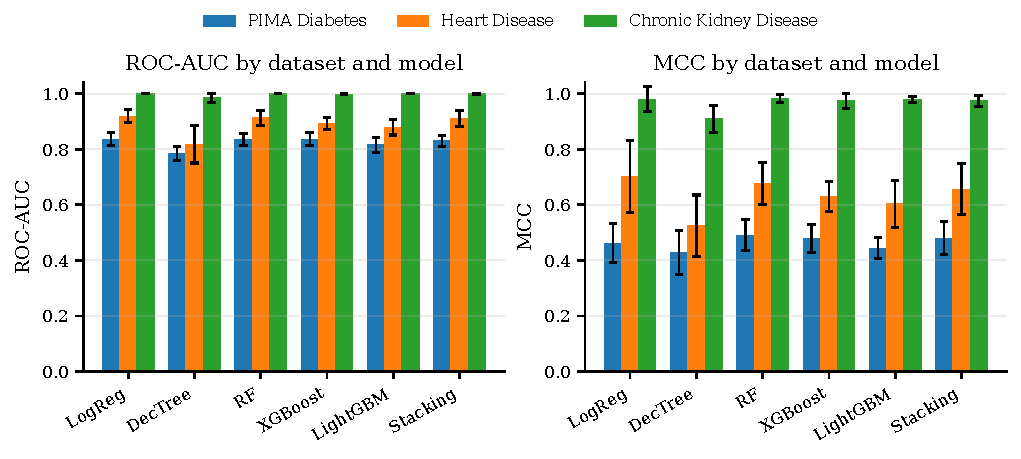
\includegraphics[width=0.88\textwidth]{F3.pdf}\end{center}
\takeaway{ROC-AUC \AucPima{} $\to$ \AucHeart{} $\to$ \AucCkd{}. Chronic Kidney is
near-separable, which turns out to matter for agreement.}
\end{frame}

\begin{frame}{RQ1: SHAP and LIME agree only moderately}
\begin{columns}[T]
\begin{column}{0.58\textwidth}
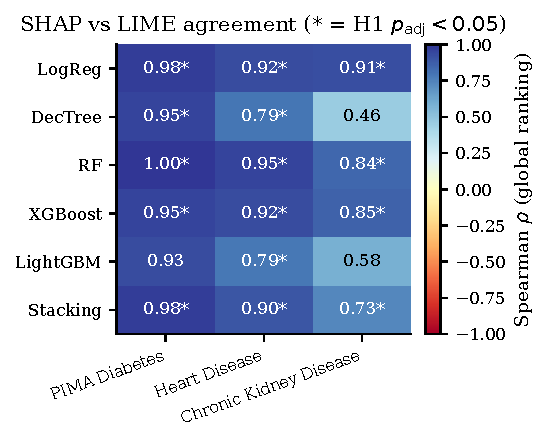
\includegraphics[width=\textwidth]{F4.pdf}
\end{column}
\begin{column}{0.4\textwidth}
\begin{itemize}\setlength\itemsep{0.5em}
  \item Median Spearman $\rho = \MedianRho{}$
  \item Median top-5 Jaccard $= \MedianJaccardFive{}$
  \item Pre-registered bar was $\rho > 0.50$; rejected in \HOneRejected{}/\HOneTotal{}
    cells
\end{itemize}
\end{column}
\end{columns}
\takeaway{On a typical instance the two methods share about half their top five features
and order them differently. Running both is not a robustness check.}
\end{frame}

\begin{frame}{RQ1: agreement does not simply follow task difficulty}
\begin{center}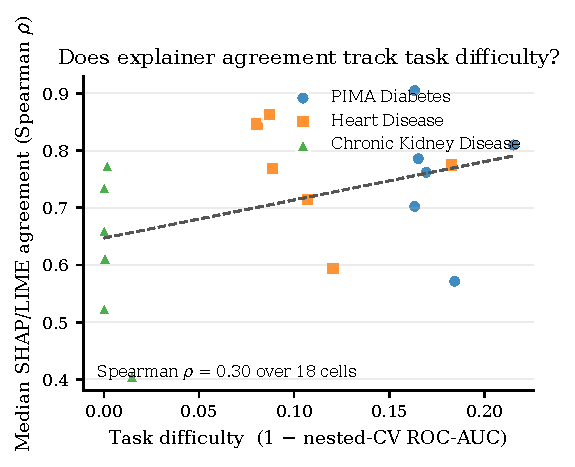
\includegraphics[width=0.62\textwidth]{F6.pdf}\end{center}
\takeaway{Our reading: agreement depends less on difficulty than on feature
\emph{redundancy}. When several features are individually sufficient, both explainers
can be locally faithful while nominating different ones.}
\end{frame}

\begin{frame}{RQ2: reproducible is not the same as robust}
\begin{columns}[T]
\begin{column}{0.5\textwidth}
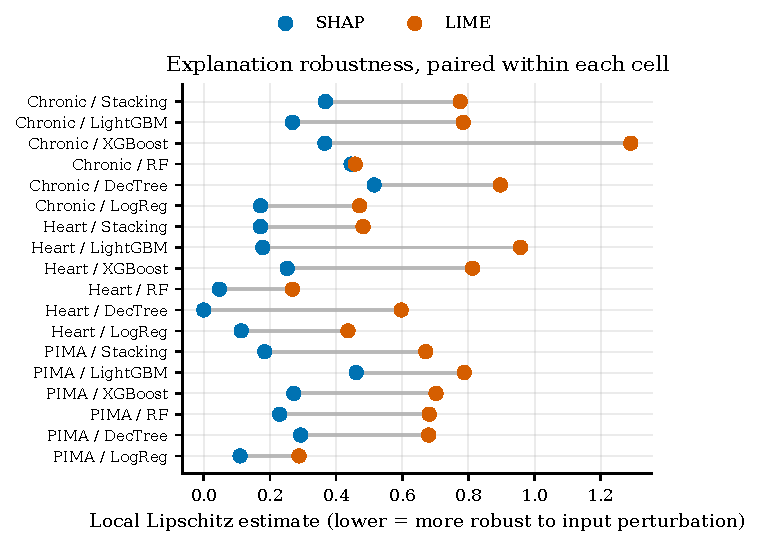
\includegraphics[width=\textwidth]{F8.pdf}
\end{column}
\begin{column}{0.48\textwidth}
\small
\begin{tabular}{@{}lrr@{}}
\toprule
Stability of & \shap{} & \lime{} \\
\midrule
Re-run (CV) & \textbf{0} & \RerunCvLime{} \\
Perturbation ($\hat L$) & \LipschitzShap{} & \LipschitzLime{} \\
Retraining ($\rho$) & \RetrainShap{} & \RetrainLime{} \\
\bottomrule
\end{tabular}
\medskip
\footnotesize Tree \shap{}'s re-run CV is \emph{exactly} zero --- declared a priori in
the protocol, not discovered.
\end{column}
\end{columns}
\takeaway{A perfectly deterministic explanation still moves when the model is refit on a
resample of the same data. That instability is in the model, and determinism cannot fix it.}
\end{frame}

\begin{frame}{RQ3: both are faithful --- and the control is why we can say so}
\begin{center}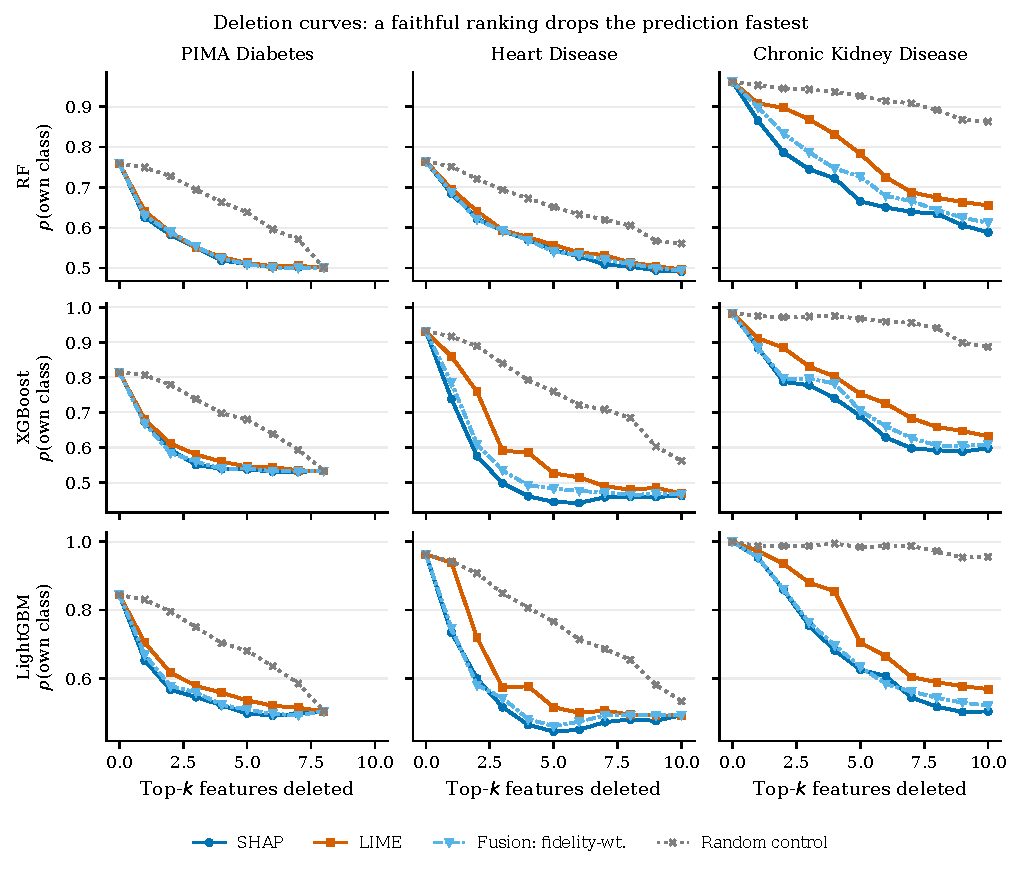
\includegraphics[width=0.82\textwidth]{F10.pdf}\end{center}
\takeaway{\aopc{}: \shap{} \AopcShap{}, \lime{} \AopcLime{}, random \AopcRandom{}.
Beat the control in \HThreeBRejected{}/\HThreeBTotal{} tests after Holm correction.}
\end{frame}

\begin{frame}{RQ4: SHAP is cheaper by roughly an order of magnitude}
\begin{center}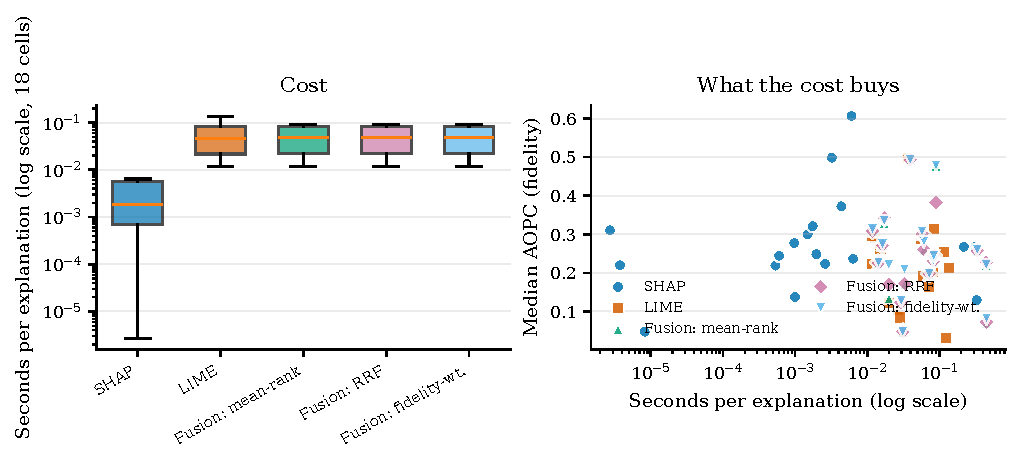
\includegraphics[width=0.9\textwidth]{F11.pdf}\end{center}
\takeaway{\SecondsShap{}\,s versus \SecondsLime{}\,s --- about
\SpeedFactor{}$\times$. Structural, not an implementation detail: \lime{} must evaluate
the model on thousands of perturbed rows per explanation.}
\end{frame}

\begin{frame}{RQ5: the plausibility check does not discriminate --- and we said so first}
\begin{center}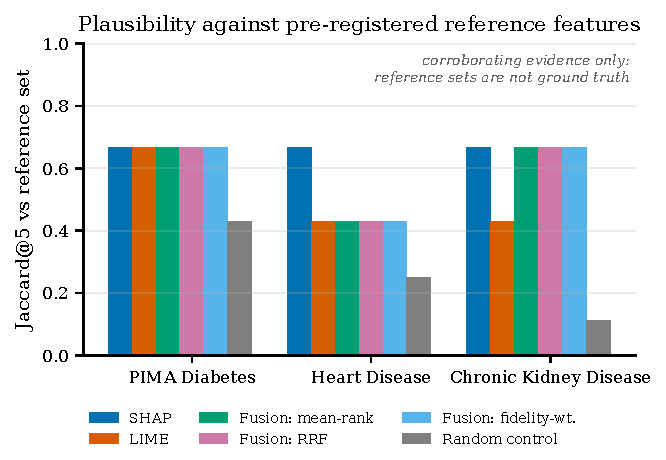
\includegraphics[width=0.68\textwidth]{F12.pdf}\end{center}
\takeaway{Both beat random; neither separates from the other. Literature-derived
reference sets are \emph{not} ground truth, and we pre-registered this as the weakest
measurement in the study.}
\end{frame}

\begin{frame}{RQ6: fusion does not clear the bar --- a pre-registered null result}
\begin{columns}[T]
\begin{column}{0.55\textwidth}
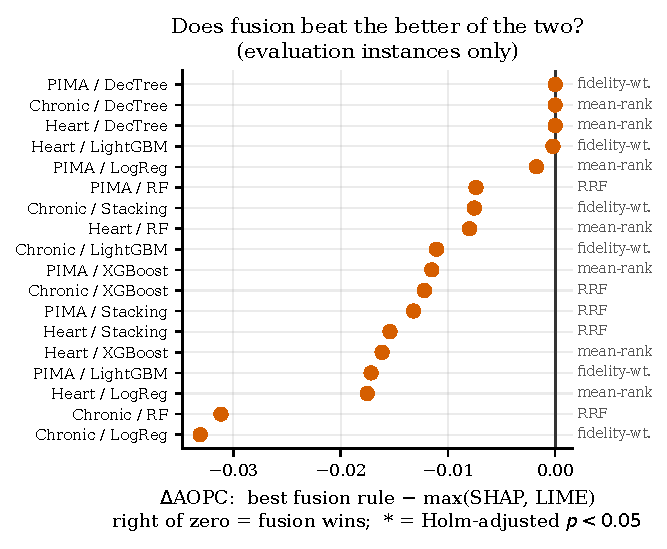
\includegraphics[width=\textwidth]{F13.pdf}
\end{column}
\begin{column}{0.43\textwidth}
\begin{itemize}\setlength\itemsep{0.5em}
  \item Bar: beat the \textbf{better} of the two, not their average
  \item Won in \HSixRejected{} of \HSixTotal{} cells
  \item Best fusion \aopc{} \AopcBestFusion{} vs \shap{} \AopcShap{}
\end{itemize}
\end{column}
\end{columns}
\takeaway{Follows from \RQ{1}: fusion needs \emph{complementary} inputs. Here the two
agree moderately and one is consistently better, so averaging moves toward the weaker.}
\end{frame}

\begin{frame}{All eleven hypotheses, auditable against the frozen protocol}
\begin{center}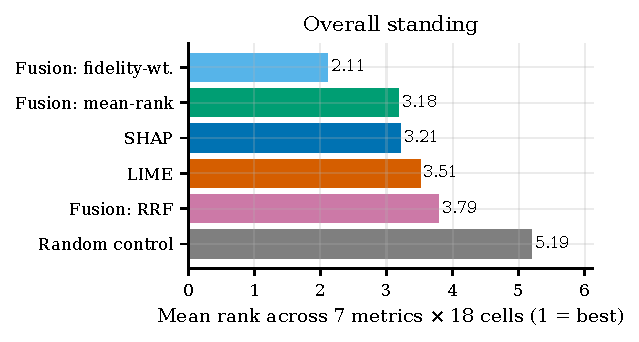
\includegraphics[width=0.62\textwidth]{F14.pdf}\end{center}
\takeaway{The protocol was committed \emph{before} any result existed, so the git
history is itself the evidence that nothing was adjusted after seeing the numbers.}
\end{frame}

\begin{frame}{Limitations --- stated before anyone has to ask}
\begin{itemize}\setlength\itemsep{0.55em}
  \item \textbf{Three datasets.} Per-cell tests have power; generalisation across
    datasets rests on three points.
  \item \textbf{Perturbation baselines are off-manifold.} A marginal-draw sensitivity
    check did not reverse the ordering, but both variants assume independence.
  \item \textbf{Reference sets are not ground truth} --- incomplete, non-causal,
    shaped by what the source literature measured.
  \item \textbf{Retraining stability covers 3 of 6 models}, restricted in advance on
    compute grounds and disclosed.
  \item \textbf{One additivity outlier retained}, not removed --- forcing that cell to
    log-odds would have been the larger distortion.
  \item \textbf{No human evaluation.} Whether an explanation helps a person decide
    better is a different question.
\end{itemize}
\end{frame}

\begin{frame}{What to take away}
\begin{enumerate}\setlength\itemsep{0.6em}
  \item \shap{} and \lime{} agree only moderately ($\rho = \MedianRho{}$) --- the choice
    of explainer is part of the decision.
  \item Where a tree backend exists, \shap{} won on fidelity, cost, and robustness.
    \lime{}'s case is model-agnosticism.
  \item Stability has three separable sources. The one a deterministic explainer cannot
    fix --- retraining variance --- is the one that matters.
  \item Rank fusion did not beat the better of the two, and the null result was
    pre-registered as valid.
\end{enumerate}
\vfill
{\small Everything reproduces with \texttt{make all}: pinned dependencies, checksummed
data, a SHA-256 per artefact, and a protocol frozen in version control.}
\end{frame}

\begin{frame}[standout]
Questions
\end{frame}

\appendix
\begin{frame}{Backup: per-instance agreement distributions}
\begin{center}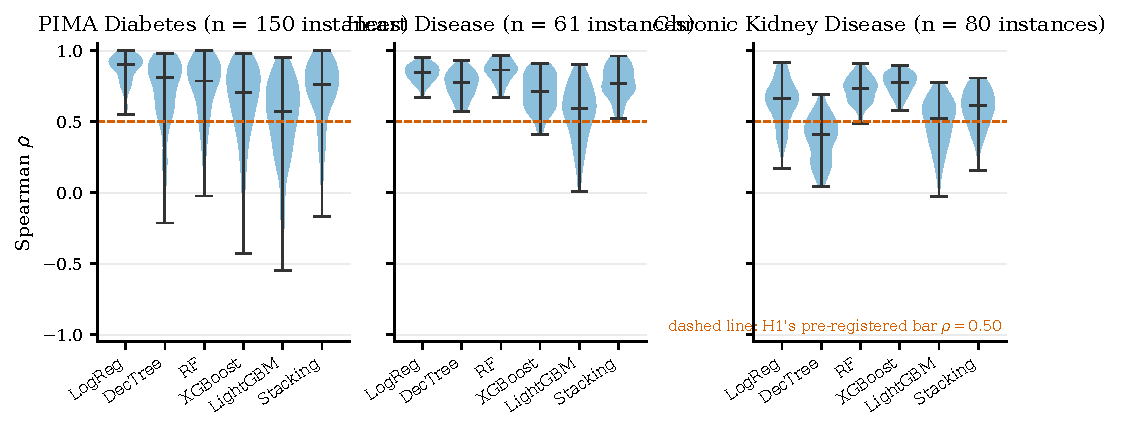
\includegraphics[width=0.95\textwidth]{F5.pdf}\end{center}
\end{frame}

\begin{frame}{Backup: LIME's variance is a budget you choose}
\begin{center}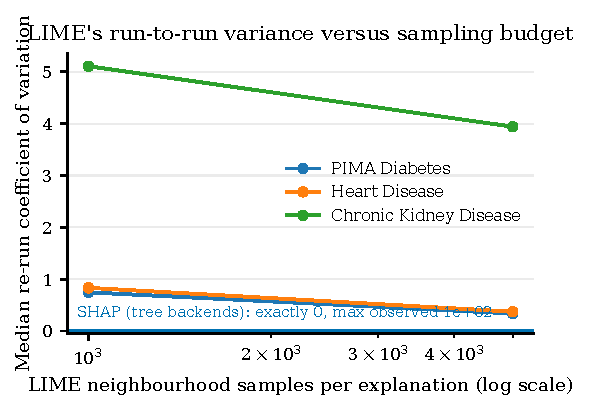
\includegraphics[width=0.62\textwidth]{F7.pdf}\end{center}
\end{frame}

\begin{frame}{Backup: retraining stability, the three ensembles}
\begin{center}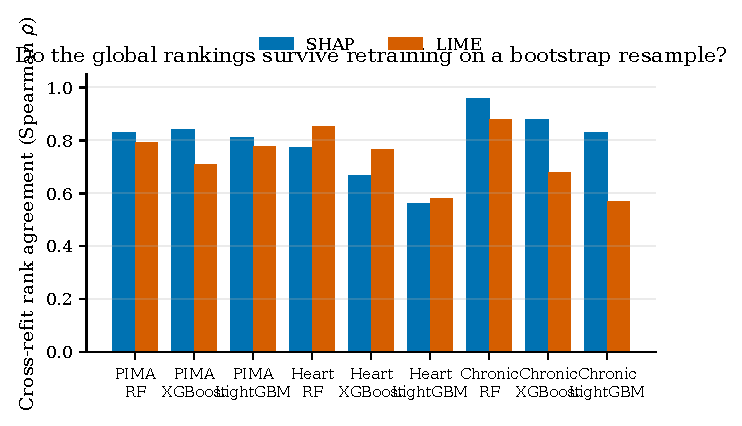
\includegraphics[width=0.78\textwidth]{F9.pdf}\end{center}
\end{frame}

\begin{frame}{Backup: dataset characteristics and missingness}
\begin{center}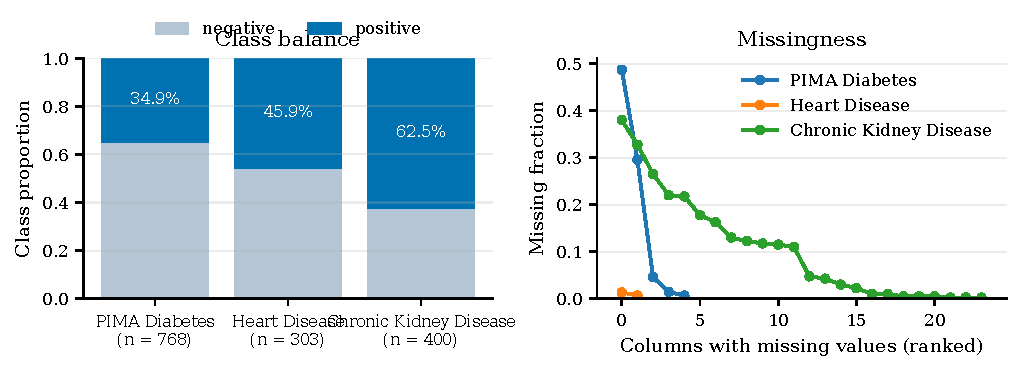
\includegraphics[width=0.95\textwidth]{F2.pdf}\end{center}
\end{frame}

\begin{frame}{Backup: ``What exactly is novel here?''}
\small
Three claims, each verifiable from a named table:
\begin{enumerate}\setlength\itemsep{0.4em}
  \item A \textbf{controlled benchmark} --- \NumCells{} cells, one protocol, 11
    pre-registered hypotheses, Holm-corrected, effect sizes and intervals throughout.
  \item A \textbf{stability decomposition} into three separable sources measured on the
    same models.
  \item A \textbf{hybrid consensus method} --- fidelity-weighted rank fusion --- against
    two published baselines and a strict bar.
\end{enumerate}
\medskip
We claim no priority for explanation aggregation itself --- that is prior work and we
cite it. Ours is the fidelity weighting, the leakage-safe calibration split, and the
controlled test. An evaluation claim cannot be refuted by a citation.
\end{frame}

\begin{frame}{Backup: ``Your SHAP stability result is trivially zero''}
\small
Correct --- and stated in the protocol \emph{before} the experiment ran, because
\textsc{TreeExplainer} is deterministic given a fixed background. Reporting it as a
discovery would be the error.
\medskip
The informative measurements are the other two:
\begin{itemize}
  \item perturbation robustness $\hat L$: \LipschitzShap{} vs \LipschitzLime{} ---
    non-trivial for both
  \item retraining stability: \RetrainShap{} vs \RetrainLime{} --- and this is where a
    deterministic explainer's guarantee runs out
\end{itemize}
The stacking cells are also informative for re-run variance, since they admit no tree
backend and \shap{} is sampling-based there.
\end{frame}

\begin{frame}{Backup: ``Isn't median imputation off-manifold?''}
\small
Yes --- Hooker et al.\ (2019) is exactly this objection, and we do not dispute it.
\medskip
Which is why every fidelity measurement is repeated with baselines drawn from each
feature's observed training marginal, so perturbed rows stay marginally plausible. The
ordering of the explainers did not reverse.
\medskip
Both variants still assume feature independence. A fully on-manifold evaluation needs a
generative model of the data, which we name as future work rather than gesture at.
\end{frame}

\begin{frame}{Backup: ``Did you correct for multiple comparisons?''}
\small
Holm--Bonferroni \emph{within} each hypothesis family --- the family being the set of
cells that hypothesis spans (18 for most, 36 for the control comparisons, 9 for
retraining). Both raw and adjusted $p$ are reported for every test; decisions use the
adjusted value.
\medskip
Degenerate cells --- those with no variation to test, expected for tree \shap{} --- are
kept in the table and reported, but excluded from the correction divisor. Correcting a
test that was never performed only discards power.
\medskip
With hundreds of instances per cell, significance is cheap. The effect size is the
finding, and it appears beside every $p$-value.
\end{frame}

\begin{frame}{Backup: ``Three datasets is not many''}
\small
Agreed, and it is the study's main limitation.
\medskip
The design compensation is the \textbf{difficulty gradient}: ROC-AUC \AucPima{} to
\AucCkd{}, which lets us ask a question a wider but flatter set of datasets could not.
\medskip
On reflection we would widen the dataset axis before the model axis --- four models
across eight datasets would support a stronger claim for the same compute. That is
recorded in the report's ``what we would do differently''.
\end{frame}

\begin{frame}{Backup: how to reproduce}
\small
\begin{itemize}\setlength\itemsep{0.4em}
  \item \texttt{make setup} --- virtualenv from \texttt{requirements.lock.txt}
  \item \texttt{make data} --- download, verify SHA-256, vendor locally
  \item \texttt{make test} --- the full suite, including metric correctness against
    analytically known answers
  \item \texttt{make smoke} --- entire pipeline plus document builds in $\sim$5 minutes
  \item \texttt{make all} --- \textsc{full} run, then paper, report, and slides
\end{itemize}
\medskip
\texttt{results/MANIFEST.json} carries a SHA-256 per artefact, the git commit, the
complete seed set, resolved library versions, and the hardware.
\end{frame}

\end{document}
